\section{Experimental Results}
\label{sec:experimental-results}

\begin{table*}[t]
  \footnotesize
  \noindent\makebox[\textwidth]{
    \begin{tabular}{ccccc}
      \toprule

      \multicolumn{1}{l}{Configuration}
      & \multicolumn{1}{l}{\# Instances solved}
      & \begin{tabular}[c]{@{}c@{}}\# Instances solved\\ (matching expected\\ solution)\end{tabular}
      & Mean Time (s)
      & \multicolumn{1}{l}{Median Time (s)}
      \\ \midrule

      S-e1:c1    & 48 & 3  & 4.62  & 0.48 \\ \midrule 
      S-e1:c2    & 49 & 6  & 0.67  & 0.29 \\ \midrule 
      S-e2:c1    & 39 & 21 & 51.28 & 3.21 \\ \midrule
      S-e2:c2    & 42 & 13 & 46.30 & 1.12 \\ \midrule
      S-e3:c1    & 34 & 23 & 51.38 & 4.47 \\ \midrule
      S-e3:c2    & 34 & 19 & 39.97 & 1.34 \\ \midrule
      W-e1:c1    & 47 & 2  & 6.76  & 0.65 \\ \midrule
      W-e1:c4    & 50 & 4  & 2.69  & 0.09 \\ \midrule
      W-e2:c1    & 13 & 4  & 11.14 & 2.24 \\ \midrule
      W-e2:c4    & 17 & 7  & 50.37 & 0.15 \\ \midrule
      W-e3:c1    & 9  & 5  & 21.45 & 7.48 \\ \midrule
      W-e3:c4    & 10 & 5  & 0.27  & 0.17 \\ \midrule
      SyPet-All  & 11 & 6  & 31.27 & 3.00 \\ \midrule
      SyPet-User & 32 & 30 & 52.75 & 5.00 \\ \bottomrule

    \end{tabular}}
  \caption{Comparison between the different configurations by number of instances
    solved and running wall-clock time for solved instances (not necessarily
    matching the expected solution).}
  \label{table:comparison-configs}
\end{table*}


A set of 285,522 expressions were provided by OutSystems.
We conducted an analysis to determine which builtin functions and which
combinations were the most common in that set.
We picked 51 expressions containing only functions from
Table~\ref{table:builtin-description}, and sizes (number of components) ranging
from 1 to 7.
The hardness of a benchmark depends on the size of the solution, the number of
input-output examples, and the library of components.
Typically, the higher the size and the number of components, the harder it is to
synthesize a program.
We obtained a set of 3 input-output examples for each of these 51 expressions.
In order to do that, we developed an \textit{interpreter} for OutSystems
expressions, and manually created a set of 3 different inputs for each
expression.
The inputs were carefully crafted in order to try to eliminate as much ambiguity
as possible.
Then we interpreted the expressions over their set of inputs in order to
obtain the corresponding outputs.

We used Z3 version 4.8.5~\cite{DeMoura:2008:ZES} as the underlying \gls{smt}
solver. 
Each benchmark was monitored by the \textit{runsolver}
program~\cite{Roussel:2011:JSAT}, and restricted to a wall-clock time limit of
600 seconds, and a memory limit of 16 GB.
We ran the experiments in an computer with Intel(R) Xeon(R) CPU E5-2620 v4 @
2.10GHz processors.

\subsection{Evaluation}
\label{sec:eval}

We are interested in the relation between the number and quality of the
input-output examples, and their impact on synthesis time and program quality.
In this section, we only study the impact of the number of input-output
examples.

We present the results for both synthesizers with the following configurations.
For each instance of 3 input-output examples we ran both synthesizers using 1,
2, or all 3 of the input-output examples.
We ran the setwise synthesizer configured to synthesize programs with a maximum
of one integer and one string constants (we refer to these configurations as
S-e1:c1, S-e2:c1, and S-e3:c1, for 1, 2, and 3 input-output examples,
respectively), and also with a maximum of two integer and two string constants
(configurations S-e1:c2, S-e2:c2, and S-e3:c2).
We ran the whole synthesizer configured to synthesize programs with a maximum of
one constant.
The synthesizer can choose whether this constant is an integer or a string
(configurations W-e1:c1, W-e2:c1, and W-e3:c1, for 1, 2, and 3 input-output
examples, respectively).
Similarly, we also run the whole synthesizer configured to use a maximum of four
constants (configurations W-e1:c4, W-e2:c4, and W-e3:c4).
For comparison, we also instantiated SyPet~\cite{Feng:2017:CSC}, a \gls{pbe}
component-based synthesizer for Java programs that employs a type-directed
search together with a constraint-based technique, with our library of
components.
However, SyPet does not support guessing the value of constants.
With this in mind, we set up two configurations for SyPet.
For the first configuration (SyPet-All), we introduced a new 0-arity component
for each constant in a pool of predefined constants.
For the second configuration (SyPet-User), we looked at each particular
instance, and introduced new components only for the constants needed for the
expected solution.
This mimics a setting where the constants are declared by the user, instead of
being guessed by the synthesizer.
Both Sypet-User and Sypet-All are configured for using all three examples of
each benchmark, and may use as many constants as they need (out of the available
ones).
Table~\ref{table:comparison-configs} shows a comparison between the different
configurations by number of instances solved and running wall-clock time (mean
and median for solved instances).
An instance is considered solved if the synthesized program satisfies the
input-output examples (but might or might not generalize).
Matching the expected solution means, that the synthesizer outputs a program
that, not only satisfies the input-output examples, but also captures the
original intent and generalizes to more examples.

% Expected comparison
\begin{figure*}
  \centering
  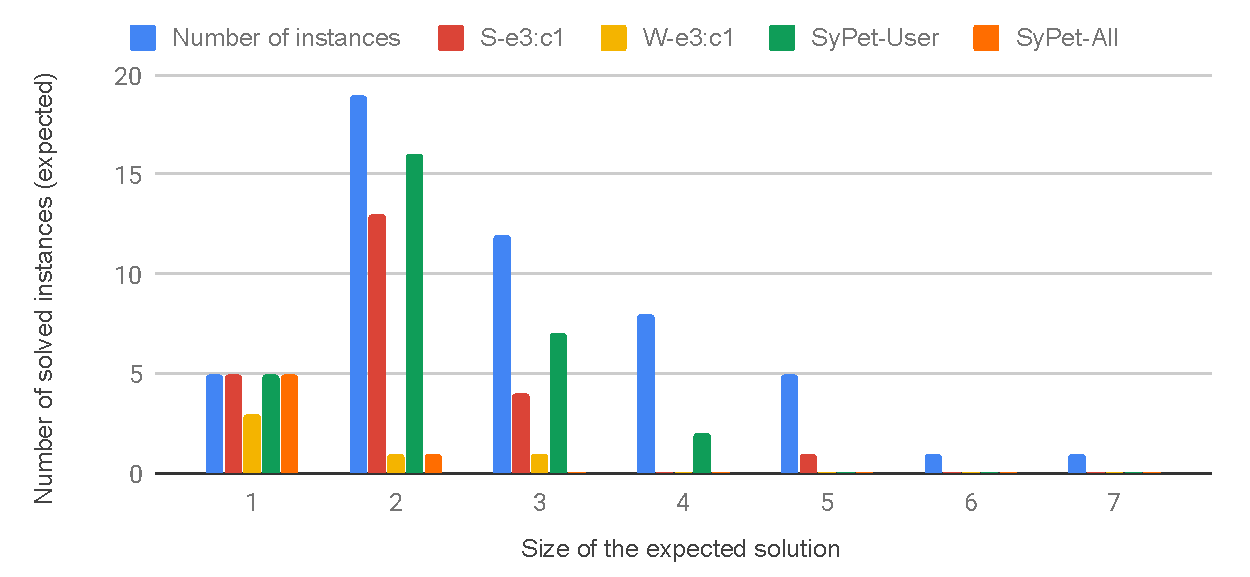
\includegraphics[scale=0.7]{assets/comparison-expected-sypet-small.pdf}
  \caption{Number of solved instances matching the expected solution per size of
    the expected solution for the setwise (one integer constant and one string
    constant) and whole synthesizers (one constant) with three examples, and
    both SyPet configurations (user-provided constants and pool of constants).}
  \label{fig:comparison-expected-sypet}
\end{figure*}

\subsection{Discussion}
\label{sec:discussion}

Figure~\ref{fig:comparison-expected-sypet} shows a comparison between all
configurations on three input-output examples.
We can see that SyPet-All has similar results to W-e3:c1.
The large number of components makes the search space intractable.
Besides, SyPet cannot take advantage of its type-directed algorithm because
we are dealing with only two types (integers and strings).
This last point also applies to SyPet-User, but the advantage given by the
user-provided constants proves crucial for its fairly good results, which are
actually better than S-e3:c1 (Table~\ref{table:comparison-configs}).

Many expected solutions require more than one constant, with some requiring more
than one constant of each type.
This could lead one to think that that is the origin of the poor performance of
the whole encoding.
However, we can see that increasing the number of available constants leads to
even worse results in both synthesizers (on these instances).
The configurations with more constants available lead to more instances solved
and in less time, but also lead to less intended solutions.
It could also be speculated from the start that the whole synthesizer would
perform worse than the setwise synthesizer.
Typically, one would expect that solving one large constraint is more expensive
than solving multiple smaller constraints.

The running times for the solved benchmarks are reasonably fast, allowing for
tolerable interaction times with the user.
However, synthesizing programs with 4 or more lines seems to be out of reach for
these configurations (Figure~\ref{fig:comparison-expected-sypet}).
